\documentclass{article}
\title{RL Entry Example Learning Note}
\author{Zhengzhong}
\date{2017.12.17}
\usepackage{amsmath}
\usepackage{graphicx}
\usepackage{subcaption}
\usepackage[margin=1in]{geometry}

\begin{document}
\maketitle

\section{2017.12.17 - Learning Maze Example}
\subsubsection{World Setting}
\subsubsection{Learning Model}
\subsubsection{Code Implementation}




\section{2017.12.17 - Entry Level Example}
\subsection{About Learning Model}
\subsubsection{Which type of RL}
Value network, Q network or policy gradient?
Answer: Q network. Each sate has 2 actions: left or right. And each action in that state has a Q value.
\subsubsection{Update Model}
\paragraph{How to make action decision} At each state, the decision is made by selection the action with the largest Q value.
\paragraph{How is the Q value calculated}
Immediately after the decision is made, its corresponding Q value is updated, based on:
\subparagraph{The immediate reward} The immediate reward $R$, is dependent on whether it is destination. If it is destination, the value is 100, otherwise it is constant negative value.
\subparagraph{The difference between the next Q and current Q}. 

In total, the Q update rule is given by:
\begin{align*}
Q(S,a) = Q(S,a) + \alpha \{R + \gamma \text{max} Q(S_a, :)-Q(S,a)\}
\end{align*}
Here $\gamma$ is chosen to be 0.9. In the equation, $R$ is determined by both $S$ and $a$. If $R$ is large, then the corresponding $Q(S,a)$ will be large, which means the action is suitable. 

Here $\gamma \text{max} Q(S_a, :)-Q(S,a)$ gives the ``difference" between the current state and the next state caused by the move. This is like an expectation of future. If this expectation is positive, it means the agent can benefit from the moving. Otherwise the agent is harmed through this movement. In this particular environment, $Q(S_a, :$ how close the agent it to the goal state.

We can imagine that under this learning scheme, the blocks near target are updated firstly, then the blocks far from the target are updated.
\subsubsection{Deterministic world or stochastic world}
This seems to be a deterministic world because the outcome cause by a certain action is deterministic.

\subsection{About Code}
\subsubsection{What is the format of q table?}
Here q$\_$table is a table generated by pd.DataFrame. Thus it is a pd.DataFrame object. The rows and columns of q$\_$table can be retrieved by using pd's API.
\begin{table}[!h]
\centering
\begin{tabular}{| l | c | r |} \hline
      & left &right     \\ \hline
  0   & 0    &   0      \\ \hline
  0   & 0    &   0      \\ \hline
  0   & 0    &   0      \\ \hline
  0   & 0    &   0      \\ \hline
  0   & 0    &   0      \\ \hline
  0   & 0    &   0      \\ \hline
\end{tabular}
\label{tab:20171217_code_q_table}
\caption{The form of q table}
\end{table}
Each row is corresponding to a state, and each column is corresponding to an action. Here we have 6 states, and each state has 2 actions. This table can be constructed by using "pd.DataFrame".
\subsubsection{q table API}
Here q$\_$table is a table generated by pd.DataFrame. Thus it is a pd.DataFrame object. The rows and columns of q$\_$table can be retrieved by using pd's API.
\paragraph{.iloc}
'loaction based indexing'. The table.iloc[x,y], where x and y are numbers. The .loc method is the same as the indexing method as the traditional array indexing.
\paragraph{.ix}
'Key indexing method'. The index of table.ix[a,b], where a and b should be the key. For example, in this tutorial, iloc[1,0] is the same as ix[a,'left'].
\subsection{Q Value Update Experiment}
In this section we tested scripts with different Q value updates policy. In experiment 1, we use the default update policy, and in experiment 2, we add an heuristic to the update rule. The action which makes the agent closer to the goal destination will get an extra rewards. In both experiments, we record the step-epoch trend and the q$\_$table after training. 

The new heuristic is given by:

\begin{align*}
Q(S,a) = Q(S,a) + \alpha \{R + \gamma \text{max} Q(S_a, :)+\frac{0.1}{S_{\text{goal}}-S_a}-Q(S,a)\}
\end{align*}

\begin{figure}
\begin{subfigure}{.5\textwidth}
  \centering
  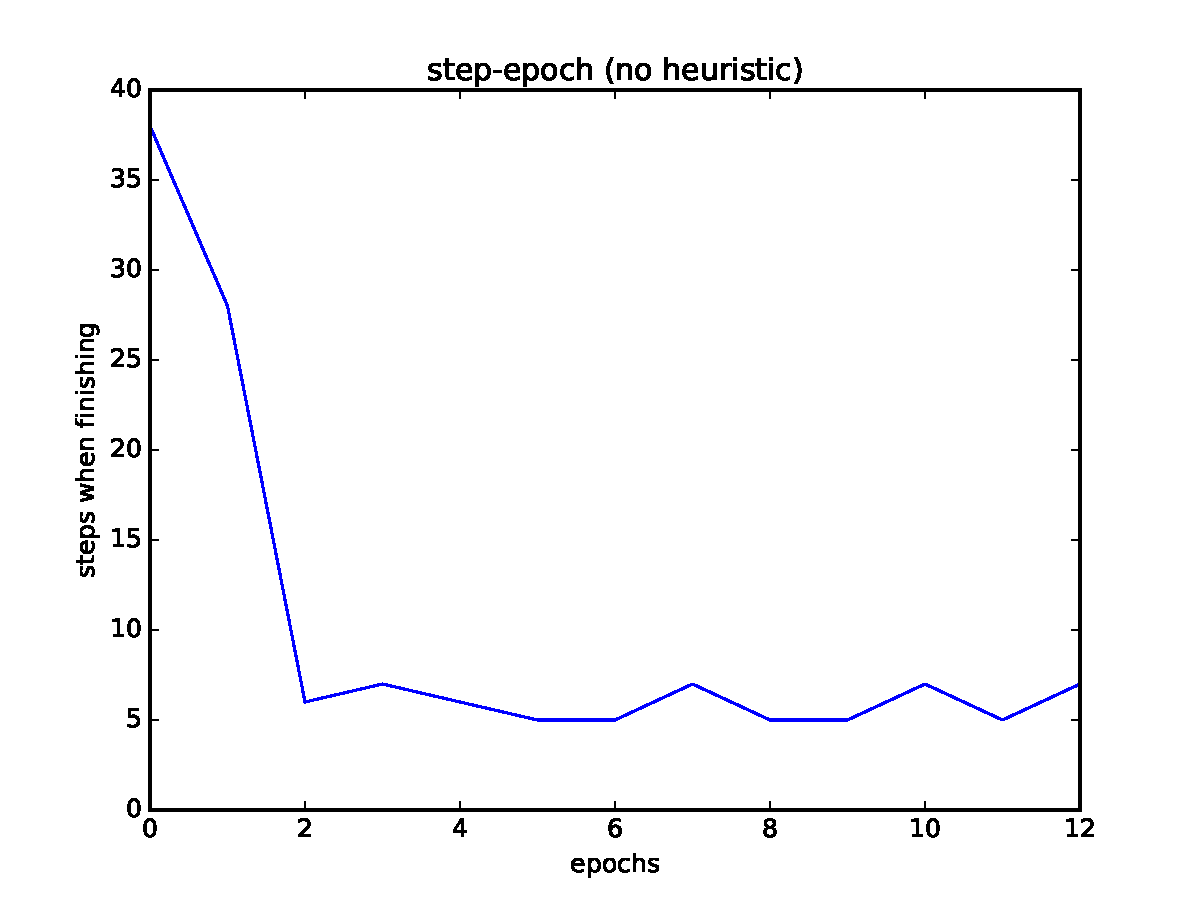
\includegraphics[width=.9\linewidth]{figures/Exp1_Q_Update_Heuristic/Steps_Heuristic_0_NoHeuristic.pdf}
  \caption{without heuristics}
  \label{fig:20171217_Q_NoHeuristic}
\end{subfigure}%
\begin{subfigure}{.5\textwidth}
  \centering
  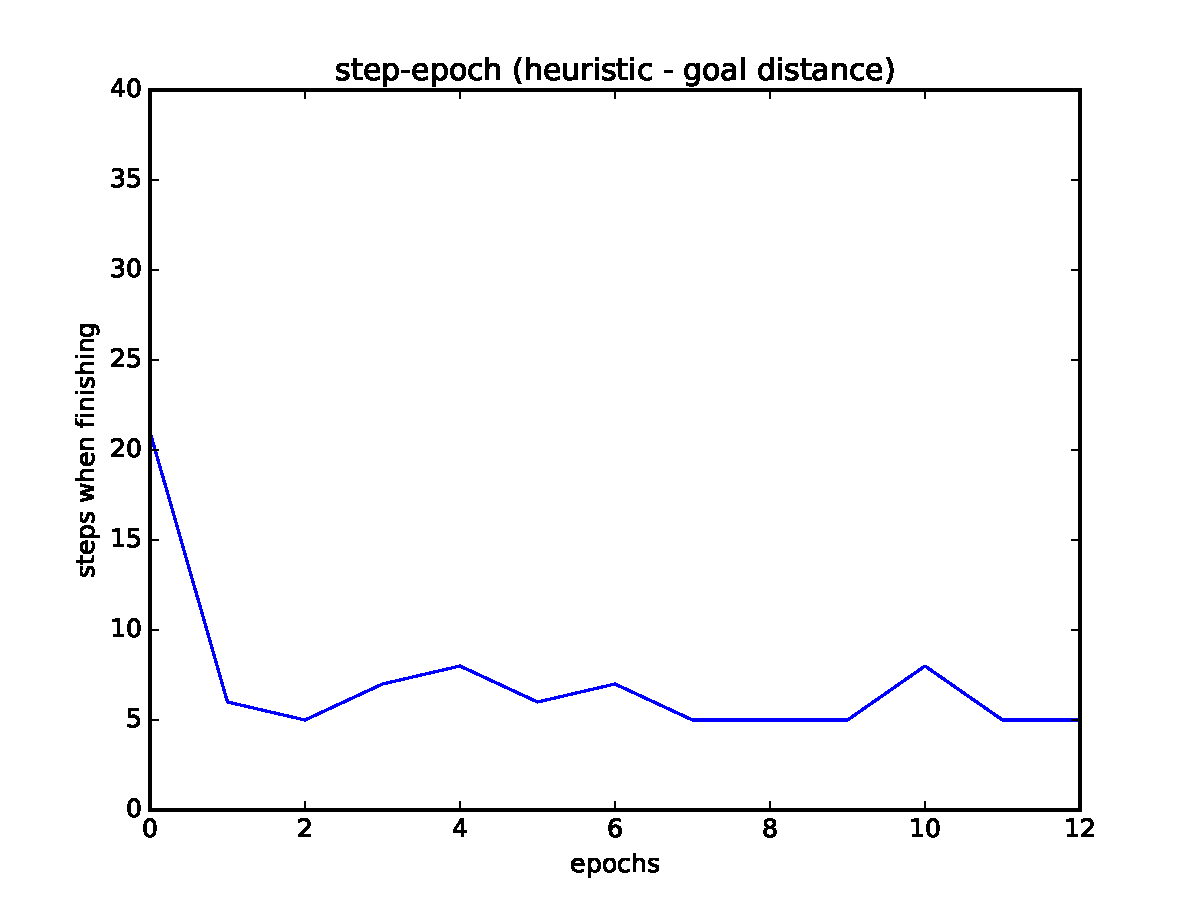
\includegraphics[width=.9\linewidth]{figures/Exp1_Q_Update_Heuristic/Steps_Heuristic_1_Distance.pdf}
  \caption{with distance heuristics}
  \label{fig:20171217_Q_Heuristic_Dist}
\end{subfigure}
\caption{Step comparison}
\label{fig:20171217_step_comparison}
\end{figure}
According to figure \ref{fig:20171217_step_comparison}, the agent will have to use less steps to reach the goal in the first 2 epochs. However, based on the new heuristic, the q value may not be able to converge because it always gets rewards for getting closer to the goal. This reward will never be 0 even in very late epochs.
\end{document}